\documentclass[11pt,a4paper]{article}

\usepackage[margin=2.5cm]{geometry}
\usepackage{amsmath,amssymb,amsthm}
\usepackage{booktabs}
\usepackage{graphicx}

\newtheorem{proposition}{Proposition}[section]
\newtheorem{theorem}[proposition]{Theorem}
\newtheorem{remark}[proposition]{Remark}
\newtheorem{conjecture}[proposition]{Conjecture}

\newcommand{\R}{\mathbb{R}}
\newcommand{\Z}{\mathbb{Z}}
\newcommand{\Q}{\mathbb{Q}}
\newcommand{\N}{\mathbb{N}}

\title{\textbf{Dual Matching Coefficients for the Continuous Hahn Weight\\
$\boldsymbol{W(x) = 2\pi^2\,\mathrm{sech}(2\pi x)}$}}
\author{Robin Langer and Claude Code}
\date{August 2026}

\begin{document}
\maketitle

%% ===================================================================
\section{The Weight and Its Polynomials}
%% ===================================================================

The continuous Hahn weight with parameters $a = c = \tfrac14$,
$b = d = \tfrac34$ is
\[
  W(x) = \Gamma(\tfrac14+ix)\,\Gamma(\tfrac34+ix)\,
         \Gamma(\tfrac14-ix)\,\Gamma(\tfrac34-ix)
       = \bigl|\Gamma(\tfrac14+ix)\,\Gamma(\tfrac34+ix)\bigr|^2.
\]
By the reflection formula, with $s = \tfrac14 + ix$:
\begin{align*}
  \Gamma(\tfrac14+ix)\,\Gamma(\tfrac34-ix)
  &= \frac{\pi}{\sin\pi(\tfrac14+ix)}, \\
  \Gamma(\tfrac34+ix)\,\Gamma(\tfrac14-ix)
  &= \frac{\pi}{\sin\pi(\tfrac34+ix)},
\end{align*}
and since
$\sin(\tfrac\pi4 + i\pi x)\,\sin(\tfrac{3\pi}{4} + i\pi x)
= \tfrac12\sin(\tfrac\pi2 + 2i\pi x)
= \tfrac12\cosh(2\pi x)$,
we obtain the elementary form
\begin{equation}\label{eq:W}
  W(x) = \frac{2\pi^2}{\cosh(2\pi x)}.
\end{equation}
This is the \emph{hyperbolic-secant weight}, an even,
rapidly decaying function with poles at $x = \pm\tfrac{i}{4} + \tfrac{in}{2}$
($n \in \Z$).

\subsection{Moments and Euler Numbers}

Since $W$ is even, all odd moments vanish. The even moments are
\begin{equation}\label{eq:mu}
  \mu_{2n} = \int_\R x^{2n}\, W(x)\, dx
  = \frac{\pi^2\, |E_{2n}|}{16^n},
\end{equation}
where $E_{2n}$ are the Euler numbers ($E_0 = 1$, $E_2 = -1$,
$E_4 = 5$, $E_6 = -61$, $E_8 = 1385$, \ldots; OEIS~A000364).

\begin{proof}[Derivation]
Substituting $u = 2\pi x$ gives
$\mu_{2n} = 2\pi^2 (2\pi)^{-(2n+1)} \int u^{2n}\,\mathrm{sech}\,u\,du$.
The known identity
$\int_\R u^{2n}\,\mathrm{sech}\,u\,du = \pi\,|E_{2n}|\,(\pi/2)^{2n}$
(which follows from the Fourier transform of $\mathrm{sech}$ being
$\pi\,\mathrm{sech}(\pi\xi/2)$ and comparing Taylor coefficients)
yields~\eqref{eq:mu} after simplification.
\end{proof}

\subsection{Monic Orthogonal Polynomials}

The monic orthogonal polynomials $p_n$ for $W$ satisfy
\begin{equation}\label{eq:rec}
  p_{n+1}(x) = x\, p_n(x) - \frac{n^2}{16}\, p_{n-1}(x),
  \qquad p_0 = 1, \quad p_1 = x.
\end{equation}
The recurrence coefficients $\alpha_n = 0$ (by evenness)
and $\beta_n = n^2/16$ were computed exactly from the
Euler-number moments via the Chebyshev algorithm with
rational arithmetic, and verified to $n = 11$.

\begin{remark}
These are rescaled Meixner--Pollaczek polynomials.
The standard monic MP($\lambda = \tfrac12$, $\phi = \tfrac\pi2$) polynomials
$q_n(y)$ satisfy $q_{n+1} = y\,q_n - (n^2/4)\,q_{n-1}$
and are orthogonal for $\mathrm{sech}(\pi y)$.
Scaling $y = 2x$ and $p_n(x) = 2^{-n} q_n(2x)$ converts
$\mathrm{sech}(\pi y)$ to $\mathrm{sech}(2\pi x)$
and $\beta_n^{\text{MP}} = n^2/4$ to $\beta_n = n^2/16$.
\end{remark}

The norms (with respect to $W/\pi^2$) are
$h_n/\pi^2 = \prod_{j=1}^n (j^2/16) = (n!)^2/16^n$,
so the orthonormal polynomials are
$\widehat{p}_n = p_n/\sqrt{h_n} = p_n \cdot 4^n/(\pi\, n!)$.

%% ===================================================================
\section{The Dual Split and Matching Matrices}
%% ===================================================================

The weight factors analytically:
\[
  W(x) = w_+(x)\, w_-(x), \qquad
  w_+(x) = \Gamma(\tfrac14+ix)\,\Gamma(\tfrac34+ix), \qquad
  w_-(x) = \overline{w_+(x)}.
\]
This defines dual functions $F_m = w_+\,\widehat{p}_m$
and $G_m = w_-\,\widehat{p}_m$ with
$\langle F_m, G_k \rangle = \delta_{mk}$.

We study two matching matrices: the \emph{orthogonal-function matching}
\[
  b_{mk} = \int_\R \widehat{p}_m(x)\,\widehat{p}_k(x)\; W(x)^{3/2}\, dx,
\]
with kernel $W^{3/2} = (2\pi^2)^{3/2}\,\mathrm{sech}(2\pi x)^{3/2}$
(which has branch points at $x = \pm i/4$), and the
\emph{dual-split matching}
\[
  c_{mk} = \int_\R \widehat{p}_m(x)\,\widehat{p}_k(x)\; w_+(x)\, W(x)\, dx,
\]
whose kernel is
$\Gamma(\tfrac14+ix)^2\,\Gamma(\tfrac34+ix)^2\,
\Gamma(\tfrac14-ix)\,\Gamma(\tfrac34-ix)$
--- a six-Gamma integral (three pairs).

By the symmetry $x \to -x$, both kernels enjoy a
\emph{checkerboard} structure:
$b_{mk} = 0$ when $m+k$ is odd (verified to $10^{-58}$),
while $c_{mk}$ is real when $m+k$ is even and purely imaginary
when $m+k$ is odd (worst violation $< 3 \times 10^{-58}$).

%% ===================================================================
\section{Barnes Evaluation of $c_{00}$}
%% ===================================================================

\begin{theorem}\label{thm:c00}
The base entry of the dual-split matching matrix is
\begin{equation}\label{eq:c00}
  c_{00} = 4\sqrt{\pi}\, U(1, 1, 2)
         = 4\sqrt{\pi}\, e^2\, E_1(2)
         = 2.56175319378357597\ldots\,,
\end{equation}
where $U$ is Tricomi's confluent hypergeometric function and
$E_1(z) = \int_z^\infty e^{-t}/t\,dt$ is the exponential integral.
\end{theorem}

\begin{proof}
Since $\widehat{p}_0 = 1/\pi$, we have
$c_{00} = (1/\pi^2)\int w_+\,W\,dx$.
Legendre's duplication formula gives
\begin{align}
  \Gamma(\tfrac14+ix)\,\Gamma(\tfrac34+ix)
  &= \sqrt{\pi}\; 2^{1/2 - 2ix}\, \Gamma(\tfrac12+2ix), \label{eq:dup1}\\
  \Gamma(\tfrac14-ix)\,\Gamma(\tfrac34-ix)
  &= \sqrt{\pi}\; 2^{1/2 + 2ix}\, \Gamma(\tfrac12-2ix). \label{eq:dup2}
\end{align}
Substituting into the six-Gamma integrand:
\[
  w_+(x)\,W(x)
  = \bigl[\sqrt\pi\; 2^{1/2-2ix}\,\Gamma(\tfrac12{+}2ix)\bigr]^2
    \cdot \sqrt\pi\; 2^{1/2+2ix}\,\Gamma(\tfrac12{-}2ix),
\]
which simplifies to
\[
  w_+\,W = \pi^{3/2} 2^{3/2} \cdot 2^{-2ix}\,
    \Gamma(\tfrac12{+}2ix)^2\,\Gamma(\tfrac12{-}2ix).
\]
The substitution $u = 2x$ then gives
\[
  \int_\R w_+\,W\,dx
  = \pi^{3/2}\sqrt{2} \int_\R
    \Gamma(\tfrac12+iu)^2\,\Gamma(\tfrac12-iu)\;
    e^{-iu\ln 2}\, du.
\]
The shifted three-Gamma integral (Proposition~2.1
of~\cite{MP}) with $a = b = c = \tfrac12$ and $s = -\ln 2$
(so $e^{-s} = 2$ and $e^{-as} = \sqrt{2}$) gives
\[
  \int_\R
  \Gamma(\tfrac12+iu)^2\,\Gamma(\tfrac12-iu)\;
  e^{-iu\ln 2}\, du
  = 2\pi\sqrt{2}\; U(1, 1, 2).
\]
Hence $\int w_+\,W\,dx = 4\pi^{5/2}\,U(1,1,2)$, and
$c_{00} = 4\sqrt{\pi}\,U(1,1,2)$.
\end{proof}

The identity $U(1,1,z) = e^z E_1(z)$ follows from the
integral representation
$U(1,1,z) = \int_0^\infty e^{-zt}/(1+t)\,dt = e^z\int_z^\infty e^{-t}/t\,dt$.

%% ===================================================================
\section{The Matching Coefficients}
%% ===================================================================

\subsection{Matrix~(a): $\mathrm{sech}^{3/2}$ kernel}

Table~\ref{tab:b} shows the $6 \times 6$ upper-left block of $b_{mk}$.
The vanishing of entries with $m+k$ odd confirms the even-weight
parity selection rule.

\begin{table}[ht]
\centering
\small
\caption{Orthogonal-function matching coefficients $b_{mk}$
($m+k$ odd entries are zero).}\label{tab:b}
\begin{tabular}{r|rrrrrr}
$b_{mk}$ & $k=0$ & $1$ & $2$ & $3$ & $4$ & $5$ \\
\hline
$m=0$ & $3.3889$ & $0$ & $-0.8216$ & $0$ & $0.4223$ & $0$ \\
$1$ & & $1.7456$ & $0$ & $-0.7759$ & $0$ & $0.4628$ \\
$2$ & & & $0.9926$ & $0$ & $-0.6059$ & $0$ \\
$3$ & & & & $0.7020$ & $0$ & $-0.4996$ \\
$4$ & & & & & $0.5319$ & $0$ \\
$5$ & & & & & & $0.4359$
\end{tabular}
\end{table}

\subsection{Matrix~(b): Six-Gamma (dual-split) kernel}

Table~\ref{tab:c} shows the $6 \times 6$ upper-left block of $c_{mk}$.
The checkerboard pattern holds: entries with $m+k$ even are real,
entries with $m+k$ odd are purely imaginary.

\begin{table}[ht]
\centering
\small
\caption{Dual-split matching coefficients $c_{mk}$
($m+k$ even: real; $m+k$ odd: displayed as coefficient of~$i$).}\label{tab:c}
\begin{tabular}{r|rrrrrr}
$c_{mk}$ & $k=0$ & $1$ & $2$ & $3$ & $4$ & $5$ \\
\hline
$m=0$ & $2.5618$ & $-1.3709$ & $-1.0109$ & $0.7799$ & $0.6420$ & $-0.5428$ \\
$1$ & & $0.5399$ & $-0.4020$ & $-0.4647$ & $0.4056$ & $0.3824$ \\
$2$ & & & $0.3483$ & $-0.1818$ & $-0.2945$ & $0.2486$ \\
$3$ & & & & $0.2654$ & $-0.0985$ & $-0.2200$ \\
$4$ & & & & & $0.2113$ & $-0.0603$ \\
$5$ & & & & & & $0.1736$
\end{tabular}
\end{table}

\subsection{Integrality: a rank-2 lattice}

In the Meixner--Pollaczek case~\cite{MP} the dual-split coefficients
lay in $\Z A \oplus \Z B$ with two Bessel generators. The analogous
statement holds here, with generators
\[
  \mathcal A = \sqrt\pi\; e^2 E_1(2) = \sqrt\pi\, U(1,1,2), \qquad
  \mathcal B = \sqrt\pi .
\]

\begin{conjecture}\label{conj:lattice}
For all $m, k$ (reading the real part when $m+k$ is even, the
imaginary part when $m+k$ is odd),
\[
  c_{mk} \in \Q\,\mathcal A + \Q\,\mathcal B .
\]
\end{conjecture}

PSLQ at 50-digit precision confirms this for all $m, k \le 5$,
with residuals below $10^{-43}$:

\begin{table}[ht]
\centering
\small
\caption{Dual-split coefficients in the lattice
$\Q\mathcal A + \Q\mathcal B$.}\label{tab:lattice}
\begin{tabular}{cl@{\qquad}cl}
\toprule
$(m,k)$ & $c_{mk}$ & $(m,k)$ & $c_{mk}$ \\
\midrule
$(0,0)$ & $4\mathcal A$                       & $(2,2)$ & $2436\mathcal A - 880\mathcal B$ \\
$(0,1)$ & $20\mathcal A - 8\mathcal B$        & $(2,3)$ & $(25660\mathcal A - 9272\mathcal B)/3$ \\
$(0,2)$ & $24\mathcal B - 68\mathcal A$       & $(2,4)$ & $(27592\mathcal B - 76364\mathcal A)/3$ \\
$(0,3)$ & $(208\mathcal B - 572\mathcal A)/3$ & $(2,5)$ & $(121952\mathcal B - 337508\mathcal A)/5$ \\
$(0,4)$ & $(1420\mathcal A - 512\mathcal B)/3$ & $(3,3)$ & $(106112\mathcal B - 293668\mathcal A)/9$ \\
$(0,5)$ & $(16172\mathcal A - 5848\mathcal B)/15$ & $(3,4)$ & $(338800\mathcal B - 937652\mathcal A)/9$ \\
$(1,1)$ & $48\mathcal B - 132\mathcal A$      & $(3,5)$ & $(13214836\mathcal A - 4774904\mathcal B)/45$ \\
$(1,2)$ & $192\mathcal B - 532\mathcal A$     & $(4,4)$ & $353540\mathcal A - 127744\mathcal B$ \\
$(1,3)$ & $(5068\mathcal A - 1832\mathcal B)/3$ & $(4,5)$ & $(9462964\mathcal A - 3419240\mathcal B)/9$ \\
$(1,4)$ & $4628\mathcal A - 1672\mathcal B$   & $(5,5)$ & $(88888528\mathcal B - 246004652\mathcal A)/75$ \\
$(1,5)$ & $(12400\mathcal B - 34316\mathcal A)/3$ & & \\
\bottomrule
\end{tabular}
\end{table}

The denominators observed ($3, 5, 9, 15, 45, 75$) are odd; a
rescaling clearing them, as in the MP case, is expected but not yet
identified.

The square root $\sqrt{\zeta'}$ in the generating function
(see \S\ref{sec:gf}) is not an obstruction but the second generator:
since $U(1,1,z) = e^z E_1(z)$ satisfies the inhomogeneous first-order
equation $y' = y - 1/z$, the derivative algebra of the full kernel
$\sqrt{z}\,U(1,1,z)$ is spanned over $\Q(z)$ by
$\{\sqrt z\, U(1,1,z),\; \sqrt z\}$ --- rank two, with the second
basis element \emph{algebraic}. This is why $\mathcal B = \sqrt\pi$
is elementary while $\mathcal A$ is transcendental.

(An earlier version of this paper reported that PSLQ finds no
relations; the failure was an artifact of the default coefficient
bound $10^3$, while the integers above reach $10^8$.)

%% ===================================================================
\section{Decay}\label{sec:decay}
%% ===================================================================

\subsection{Matrix~(a)}

The entries $b_{0k}$ for even $k$ decay slowly:
\[
  |b_{0,0}| = 3.389, \quad
  |b_{0,2}| = 0.822, \quad
  |b_{0,4}| = 0.422, \quad
  |b_{0,6}| = 0.275, \quad
  |b_{0,8}| = 0.201.
\]
The ratios $|b_{0,2(n+1)}|/|b_{0,2n}|$ converge to approximately
$0.73$, consistent with \textbf{power-law decay} $|b_{0,k}| \sim k^{-\alpha}$
with $\alpha \approx 0.7$.
The branch point of $\mathrm{sech}(2\pi x)^{3/2}$ at $x = i/4$
is at distance $1/4$ from the real axis, but the polynomial
growth of $\widehat{p}_k$ prevents geometric decay.

\subsection{Matrix~(b)}

The entries $|c_{0,k}|$ alternate in magnitude (real vs.\ imaginary
parts) and decay slowly:
\[
  |c_{0,0}| = 2.562, \;
  |c_{0,1}| = 1.371, \;
  |c_{0,2}| = 1.011, \;
  \ldots, \;
  |c_{0,9}| = 0.337.
\]
The successive ratios converge toward $0.90$--$0.91$, suggesting
\textbf{power-law decay} $|c_{0,k}| \sim k^{-\beta}$ with
$\beta \approx 0.4$. This is significantly slower than geometric
decay and contrasts with the MP $\lambda = \tfrac14$ case where
the ratios also converge to a constant below~$1$ but were faster.

%% ===================================================================
\section{Generating Function}\label{sec:gf}
%% ===================================================================

The Meixner--Pollaczek generating function
$\sum_n P_n^{(1/2)}(y;\tfrac\pi2)\, w^n
= (1+w^2)^{-1/2}\,\varphi(w)^{-iy}$,
where $\varphi(w) = (1+iw)/(1-iw)$ is the Cayley transform
and $P_n^{(1/2)}(2x)$ is related to our $p_n(x)$ by
$P_n(2x) = 4^n/(n!)\, p_n(x)$,
allows us to sum the double generating function
\[
  \sum_{m,k \ge 0} I_{mk}\, w^m u^k
  = \int_\R \frac{w_+(x)\,W(x)}{(1+w^2)^{1/2}\,(1+u^2)^{1/2}}\;
    \varphi(w)^{-2ix}\,\varphi(u)^{-2ix}\, dx,
\]
where $I_{mk} = \int P_m(2x)\,P_k(2x)\; w_+\,W\, dx$.
After the duplication reduction of~\S3, this becomes a
shifted three-Gamma integral with shift parameter
$\zeta' = 2\,\varphi(w)\,\varphi(u)$,
yielding
\begin{equation}\label{eq:gf}
  \sum_{m,k} I_{mk}\, w^m u^k
  = \frac{4\pi^{5/2}\,\sqrt{\zeta'/2}\; U(1, 1, \zeta')}
         {\sqrt{(1+w^2)(1+u^2)}}
\end{equation}
(normalisation verified numerically against the coefficient table
to ten digits at $(w,u) = (0.1, 0.15)$). At $w = u = 0$,
$\zeta' = 2$, recovering $I_{00} = 4\pi^{5/2}\, U(1,1,2)$ and hence
$c_{00} = I_{00}/\pi^2 = 4\sqrt\pi\, U(1,1,2)$.

The matching coefficients are $c_{mk} = I_{mk}/\pi^2$
(the conversion factors between $P_n$ and $\widehat{p}_n$ cancel
because $\sqrt{h_m h_k} = \pi^2 m!\,k!/4^{m+k}$ exactly absorbs
the $4^{m+k}/(m!\,k!)$ from $P_n = (4^n/n!)\,p_n$).

\begin{remark}[Comparison with the MP case]
The MP generating function~\cite{MP} had the form
$e^{\zeta/2}\,K_0(\zeta/2)/\sqrt{(1-iw)(1-iu)}$, whose kernel
generates an \emph{irreducible} rank-2 module with basis
$\{K_0, K_1\}$: both generators $A, B$ are transcendental Bessel
values. Here the kernel $\sqrt{z}\,U(1,1,z)$ also generates a rank-2
module, $\{\sqrt z\,U(1,1,z), \sqrt z\}$, but a \emph{reducible} one
($e^z E_1(z)$ is an extension of the trivial equation by a Kummer
equation), and the reducibility is visible in the lattice: the
second generator degenerates to the elementary constant
$\mathcal B = \sqrt\pi$. In both cases the rank of the lattice
equals the rank of the derivative module of the full kernel,
prefactor included.
\end{remark}

%% ===================================================================
\section{Combinatorics}
%% ===================================================================

The Euler-number moments $\mu_{2n}/\pi^2 = |E_{2n}|/16^n$
connect the recurrence to the theory of alternating permutations:
$|E_{2n}|$ counts the number of alternating permutations of
$\{1, \ldots, 2n\}$.

The coefficients $\beta_n = n^2/16$ (equivalently
$16\beta_n = n^2$, OEIS~A000290) identify the weight
with the $\lambda = \tfrac12$ MP family.

The first few Euler numbers determining the moments:
\[
  |E_0| = 1, \quad |E_2| = 1, \quad |E_4| = 5, \quad
  |E_6| = 61, \quad |E_8| = 1385, \quad |E_{10}| = 50521.
\]

%% ===================================================================
\section{Zeros}
%% ===================================================================

Figure~\ref{fig:zeros} shows the zeros of the truncated dual functions
$\sum_{k \le N} c_{0k}\,\widehat{p}_k(z)$ and
$\sum_{k \le N} b_{0k}\,\widehat{p}_k(z)$ in the complex plane,
for $N = 8, 10, 12$.

\begin{figure}[ht]
\centering
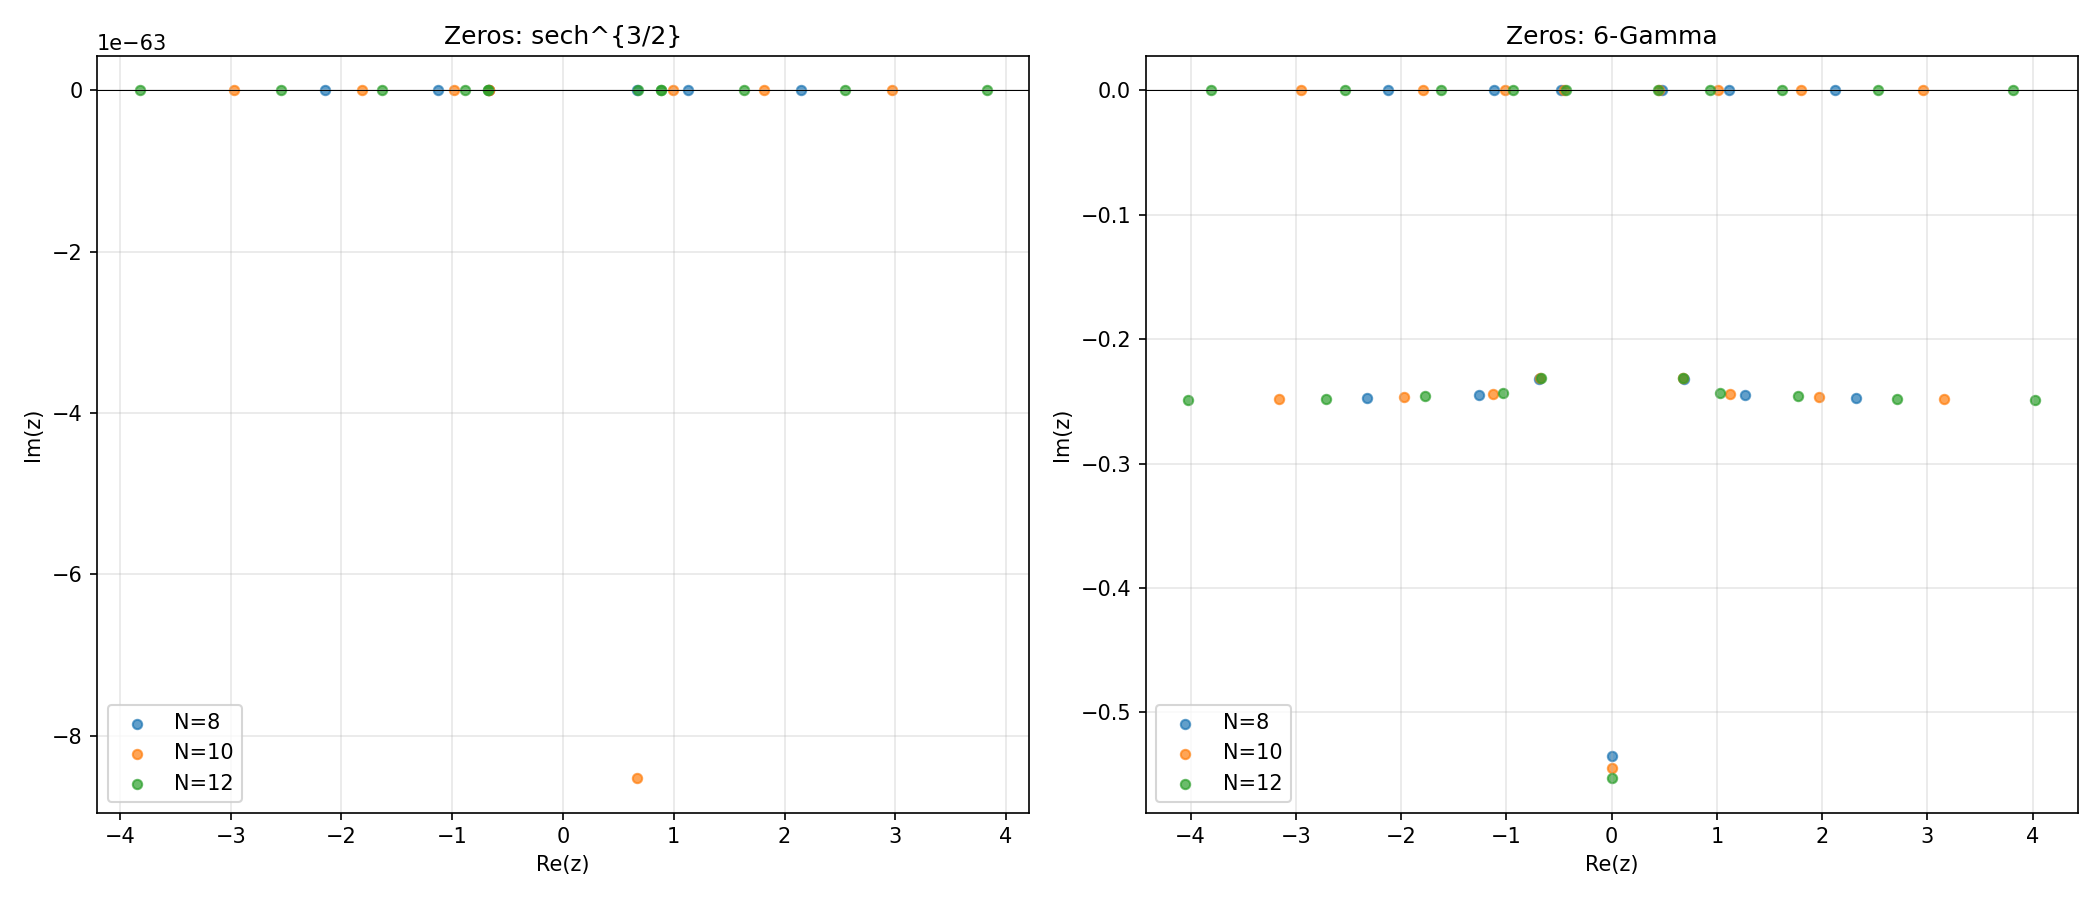
\includegraphics[width=0.95\textwidth]{hahn_zeros.png}
\caption{Zeros of the truncated dual functions. Left:
$\mathrm{sech}^{3/2}$ kernel (all zeros real). Right: six-Gamma
kernel (real and complex zeros).}\label{fig:zeros}
\end{figure}

The $\mathrm{sech}^{3/2}$ zeros are all real, as expected from a
positive kernel. The six-Gamma zeros exhibit both real zeros and
complex conjugate pairs; as $N$ increases, additional pairs appear,
but there is no clear convergence toward a limiting imaginary part
(contrast with the MP $\lambda = \tfrac14$ case where zeros converged
to $\mathrm{Im}\,x = -\tfrac12$).

%% ===================================================================
\section{Summary}
%% ===================================================================

\begin{enumerate}
\item The continuous Hahn weight $W = 2\pi^2\,\mathrm{sech}(2\pi x)$
has orthogonal polynomials with the exact recurrence
$\beta_n = n^2/16$, identified as rescaled
Meixner--Pollaczek($\lambda = \tfrac12$, $\phi = \pi/2$).

\item The duplication formula reduces the six-Gamma dual-split
integral to a three-Gamma integral, and the shifted three-Gamma lemma
gives the \textbf{closed form}
$c_{00} = 4\sqrt{\pi}\, e^2\, E_1(2)$.

\item The dual-split coefficients lie in the \textbf{rank-2 lattice}
$\Q\,\mathcal A + \Q\,\mathcal B$ with
$\mathcal A = \sqrt\pi\, e^2 E_1(2)$, $\mathcal B = \sqrt\pi$
(verified by PSLQ for $m,k \le 5$). The $\sqrt{\zeta'}$ prefactor
supplies the second, algebraic generator: the lattice rank equals
the rank of the derivative module of the kernel
$\sqrt z\, U(1,1,z)$, and the reducibility of that module is why
$\mathcal B$ is elementary.

\item Both matching matrices exhibit \textbf{power-law decay},
not geometric: $|b_{0,k}| \sim k^{-0.7}$,
$|c_{0,k}| \sim k^{-0.4}$.
\end{enumerate}

\begin{thebibliography}{9}
\bibitem{MP}
R.~Langer and Claude Code,
\emph{The Dual Meixner--Pollaczek Matching Coefficients: the Calculation},
manuscript, August 2026.
\end{thebibliography}

\end{document}
